% Options for packages loaded elsewhere
\PassOptionsToPackage{unicode}{hyperref}
\PassOptionsToPackage{hyphens}{url}
%
\documentclass[
]{article}
\usepackage{amsmath,amssymb}
\usepackage{iftex}
\ifPDFTeX
  \usepackage[T1]{fontenc}
  \usepackage[utf8]{inputenc}
  \usepackage{textcomp} % provide euro and other symbols
\else % if luatex or xetex
  \usepackage{unicode-math} % this also loads fontspec
  \defaultfontfeatures{Scale=MatchLowercase}
  \defaultfontfeatures[\rmfamily]{Ligatures=TeX,Scale=1}
\fi
\usepackage{lmodern}
\ifPDFTeX\else
  % xetex/luatex font selection
\fi
% Use upquote if available, for straight quotes in verbatim environments
\IfFileExists{upquote.sty}{\usepackage{upquote}}{}
\IfFileExists{microtype.sty}{% use microtype if available
  \usepackage[]{microtype}
  \UseMicrotypeSet[protrusion]{basicmath} % disable protrusion for tt fonts
}{}
\makeatletter
\@ifundefined{KOMAClassName}{% if non-KOMA class
  \IfFileExists{parskip.sty}{%
    \usepackage{parskip}
  }{% else
    \setlength{\parindent}{0pt}
    \setlength{\parskip}{6pt plus 2pt minus 1pt}}
}{% if KOMA class
  \KOMAoptions{parskip=half}}
\makeatother
\usepackage{xcolor}
\usepackage{longtable,booktabs,array}
\usepackage{calc} % for calculating minipage widths
% Correct order of tables after \paragraph or \subparagraph
\usepackage{etoolbox}
\makeatletter
\patchcmd\longtable{\par}{\if@noskipsec\mbox{}\fi\par}{}{}
\makeatother
% Allow footnotes in longtable head/foot
\IfFileExists{footnotehyper.sty}{\usepackage{footnotehyper}}{\usepackage{footnote}}
\makesavenoteenv{longtable}
\usepackage{graphicx}
\makeatletter
\def\maxwidth{\ifdim\Gin@nat@width>\linewidth\linewidth\else\Gin@nat@width\fi}
\def\maxheight{\ifdim\Gin@nat@height>\textheight\textheight\else\Gin@nat@height\fi}
\makeatother
% Scale images if necessary, so that they will not overflow the page
% margins by default, and it is still possible to overwrite the defaults
% using explicit options in \includegraphics[width, height, ...]{}
\setkeys{Gin}{width=\maxwidth,height=\maxheight,keepaspectratio}
% Set default figure placement to htbp
\makeatletter
\def\fps@figure{htbp}
\makeatother
\setlength{\emergencystretch}{3em} % prevent overfull lines
\providecommand{\tightlist}{%
  \setlength{\itemsep}{0pt}\setlength{\parskip}{0pt}}
\setcounter{secnumdepth}{-\maxdimen} % remove section numbering
\ifLuaTeX
  \usepackage{selnolig}  % disable illegal ligatures
\fi
\usepackage{bookmark}
\IfFileExists{xurl.sty}{\usepackage{xurl}}{} % add URL line breaks if available
\urlstyle{same}
\hypersetup{
  pdftitle={Pairwise Local Phase Summaries in Measurement-Limited Statevector Simulation Under Continuous Phase-Kick Noise},
  pdfauthor={Amy McBride},
  hidelinks,
  pdfcreator={LaTeX via pandoc}}

\title{Pairwise Local Phase Summaries in Measurement-Limited Statevector
Simulation Under Continuous Phase-Kick Noise}
\author{Amy McBride}
\date{2026-04-02}

\begin{document}
\maketitle

\textbf{Affiliation:} Independent Artist and Independent Researcher

\subsection{Abstract}\label{abstract}

This paper documents a repeated-seed statevector simulation study of
measurement-limited feedback control under continuous phase-kick noise.
Two nearest-neighbor chain workloads were evaluated: a 6-qubit chain and
a 12-qubit chain. Three controller modes were compared: no correction
(OFF), a controller using only single-qubit summaries (SINGLE\_BLOCK),
and a controller using single-qubit plus nearest-neighbor pairwise
summaries (PAIR\_BLOCK). Physical noise schedules were matched across
controller modes on a per-seed basis, and measurement randomness used a
separate random-number stream so that controller operation could not
alter the underlying noise sequence. The primary endpoint was
cycles-to-threshold, defined as the first cycle at which fidelity to the
ideal noiseless trajectory fell below 0.90.

The study was designed to answer a narrow question: when phase drift
includes nearest-neighbor structure, do nearest-neighbor pairwise
summaries expose control-relevant information that is not available from
single-qubit summaries alone? In the preserved simulation outputs
analyzed here, PAIR\_BLOCK produced longer median cycles-to-threshold
than OFF and SINGLE\_BLOCK across both workloads under independent
continuous Z kicks and under mixed phase-kick noise. Under
nearest-neighbor ZZ kicks, the advantage remained present but smaller.
The paper reports the simulation design, observable algebra, statistical
protocol, preserved results, and limits of interpretation. The scope of
the result is restricted to the measurement-limited statevector
simulation and the specific controller and noise models archived with
the run artifacts.

\subsection{1. Introduction}\label{introduction}

Measurement-based feedback is a standard tool in quantum control, and
the literature on continuous quantum measurement and feedback provides
the background for stabilizing phase-sensitive dynamics in noisy quantum
systems {[}1,2{]}. Experimental demonstrations of real-time quantum
feedback have shown that partial measurement records can be used to
stabilize target behavior in both cavity and superconducting-qubit
settings {[}3,4{]}. This paper stays within simulation, but it asks a
closely related and more specific question: if local phase drift
contains nearest-neighbor structure, what information must a controller
observe in order to respond to that structure?

The emphasis here is explanatory rather than promotional. The objective
is not to claim a new hardware protocol, a compiler advantage, or new
physics. The objective is to describe what was actually tested in a
preserved run archive, why the pairwise summaries are informative from
the Pauli algebra, and what the saved outputs show under a tightly
defined repeated-seed protocol.

\subsection{2. Simulation design}\label{simulation-design}

\subsubsection{2.1 Workloads}\label{workloads}

Two workloads were evaluated.

\begin{itemize}
\tightlist
\item
  \textbf{W6\_6q:} a 6-qubit nearest-neighbor chain with edges
  \((1,2),(2,3),(3,4),(4,5),(5,6)\).
\item
  \textbf{W12\_12q:} a 12-qubit nearest-neighbor chain with edges
  \((1,2),\ldots,(11,12)\).
\end{itemize}

For each cycle \(t\), the simulated state \(|\psi_t\rangle\) was
compared with an ideal noiseless reference state
\(|\psi_t^{\mathrm{ideal}}\rangle\) produced by running the same cycle
schedule without noise. The saved artifacts preserve the run-level
cycles-to-threshold values and final fidelity values, together with
aggregate summaries and paired comparison tables.

\subsubsection{2.2 Noise models}\label{noise-models}

All noise was applied once per cycle.

\textbf{Independent Z kicks (Z\_kick\_mid)}

\[
\theta_i(t) \sim \mathcal{N}(0,\sigma_Z^2), \qquad \sigma_Z = 0.06 \; \mathrm{rad/cycle}.
\]

\textbf{Nearest-neighbor ZZ kicks (ZZcorr\_kick\_mid)}

\[
\theta_{ij}(t) \sim \mathcal{N}(0,\sigma_{ZZ}^2), \qquad \sigma_{ZZ} = 0.06 \; \mathrm{rad/cycle}
\]

for \((i,j)\) on chain edges.

\textbf{Mixed phase-kick noise (MIX\_kick\_std)}

\begin{itemize}
\tightlist
\item
  independent Z kicks with \(\sigma_Z = 0.04\) rad/cycle,
\item
  nearest-neighbor ZZ kicks with \(\sigma_{ZZ} = 0.03\) rad/cycle,
\item
  rare X flips with probability \(p_X = 0.001\) per qubit per cycle.
\end{itemize}

The per-cycle noise unitary was

\[
U_{\mathrm{noise}}(t) =
\left[ \prod_i e^{-i\theta_i(t) Z_i / 2} \right]
\left[ \prod_{(i,j)} e^{-i\theta_{ij}(t) Z_i Z_j / 2} \right]
\left[ \prod_i X_i^{b_i(t)} \right],
\]

where \(b_i(t) \sim \mathrm{Bernoulli}(p_X)\) in the mixed condition and
\(b_i(t)=0\) otherwise.

The final study used continuous phase-kick noise rather than discrete
Pauli sign flips because the controller family tested here is based on
phase summaries; a continuous kick model supplies an observable phase
offset that such summaries can, in principle, sense.

\subsubsection{2.3 Controller modes}\label{controller-modes}

Three controller modes were compared.

\begin{itemize}
\tightlist
\item
  \textbf{OFF:} no correction.
\item
  \textbf{SINGLE\_BLOCK:} measurement-limited feedback using only
  single-qubit \(X_i\) and \(Y_i\) summaries.
\item
  \textbf{PAIR\_BLOCK:} measurement-limited feedback using single-qubit
  summaries plus nearest-neighbor pairwise summaries derived from
  \(Y_i Z_j\) and \(Z_i Y_j\) correlators.
\end{itemize}

Both active controllers used proportional correction from summary
residuals relative to the ideal target summaries preserved by the
simulation protocol. The archived configuration specifies:

\begin{itemize}
\tightlist
\item
  control update interval: every 2 cycles,
\item
  effective shot budget: 512 shots per required observable,
\item
  Gaussian finite-shot approximation,
\item
  local gain \(g_{\mathrm{local}} = 1.0\),
\item
  edge gain \(g_{\mathrm{edge}} = 0.5\).
\end{itemize}

The finite-shot approximation was implemented as

\[
\hat{\mu} = \mu + \varepsilon, \qquad
\varepsilon \sim \mathcal{N}\left(0, \frac{1-\mu^2}{N}\right), \qquad N=512.
\]

Block localization was fixed as follows.

\begin{itemize}
\tightlist
\item
  W6\_6q: 3 blocks of 2 qubits.
\item
  W12\_12q: 4 blocks of 3 qubits.
\end{itemize}

\subsubsection{2.4 Matched-seed protocol and
endpoint}\label{matched-seed-protocol-and-endpoint}

For each seed \(s\), all controller modes were run under the same
physical noise schedule. Measurement randomness was generated from a
separate random-number stream so that turning measurement or feedback on
could not change the future physical noise sequence by consuming random
draws in a different order. This separation matters, because coupled
noise and measurement RNG streams can create spurious controller
advantages.

The primary endpoint was \textbf{cycles-to-threshold},

\[
t^* = \min \{ t : F_t < 0.90 \},
\]

where

\[
F_t = |\langle \psi_t^{\mathrm{ideal}} | \psi_t \rangle|^2
\]

is fidelity to the ideal noiseless trajectory at cycle \(t\).

\subsection{3. Observable algebra}\label{observable-algebra}

The algebraic rationale for pairwise summaries is straightforward. Let

\[
U(\theta) = e^{-i\theta Z_i Z_j / 2}.
\]

Using the Pauli commutation relations,

\[
[Z_i, X_i] = 2iY_i,
\]

and therefore

\[
[Z_i Z_j, X_i] = Z_j[Z_i,X_i] = 2i Y_i Z_j,
\]

\[
[Z_i Z_j, X_j] = Z_i[Z_j,X_j] = 2i Z_i Y_j.
\]

Repeated commutators close on two-dimensional subspaces,

\[
[Z_i Z_j, Y_i Z_j] = -2i X_i,
\]

with an analogous closure for the \((X_j, Z_i Y_j)\) pair. Conjugation
then yields

\[
U(\theta)^\dagger X_i U(\theta) = X_i \cos\theta + (Y_i Z_j) \sin\theta,
\]

\[
U(\theta)^\dagger X_j U(\theta) = X_j \cos\theta + (Z_i Y_j) \sin\theta.
\]

A nearest-neighbor \(ZZ\) phase perturbation therefore rotates
single-qubit \(X\) components into pairwise \(YZ\) and \(ZY\)
correlators. A controller restricted to single-qubit summaries cannot
directly observe the full response generated by a \(ZZ\) phase term.
Pairwise summaries are informative because they expose the edge-phase
component that single-qubit summaries alone leave partially hidden.

\subsection{4. Statistical protocol}\label{statistical-protocol}

For each comparison and seed, a paired delta was formed,

\[
\Delta_s = t^*_{A,s} - t^*_{B,s}.
\]

The main analysis reports median cycles, mean cycles, interquartile
range (IQR), and standard deviation for each controller mode and
condition. For paired comparisons, the archived results report the
paired median delta, paired mean delta, positive/negative/zero fractions
across seeds, and a 95\% percentile bootstrap confidence interval for
the paired median delta using 5000 bootstrap resamples {[}5{]}.

The main benchmark used 80 matched seeds. A separate sensitivity pass
used 80 fresh system-entropy seeds for OFF and PAIR\_BLOCK under the
same workload and noise combinations.

\subsection{5. Results}\label{results}

\subsubsection{5.1 Descriptive summaries}\label{descriptive-summaries}

\textbf{Table 1. W6\_6q descriptive statistics}

\begin{longtable}[]{@{}
  >{\raggedright\arraybackslash}p{(\columnwidth - 10\tabcolsep) * \real{0.2935}}
  >{\raggedright\arraybackslash}p{(\columnwidth - 10\tabcolsep) * \real{0.1522}}
  >{\raggedleft\arraybackslash}p{(\columnwidth - 10\tabcolsep) * \real{0.1848}}
  >{\raggedleft\arraybackslash}p{(\columnwidth - 10\tabcolsep) * \real{0.1630}}
  >{\raggedright\arraybackslash}p{(\columnwidth - 10\tabcolsep) * \real{0.1413}}
  >{\raggedleft\arraybackslash}p{(\columnwidth - 10\tabcolsep) * \real{0.0652}}@{}}
\toprule\noalign{}
\begin{minipage}[b]{\linewidth}\raggedright
Noise
\end{minipage} & \begin{minipage}[b]{\linewidth}\raggedright
Mode
\end{minipage} & \begin{minipage}[b]{\linewidth}\raggedleft
Median cycles
\end{minipage} & \begin{minipage}[b]{\linewidth}\raggedleft
Mean cycles
\end{minipage} & \begin{minipage}[b]{\linewidth}\raggedright
IQR
\end{minipage} & \begin{minipage}[b]{\linewidth}\raggedleft
SD
\end{minipage} \\
\midrule\noalign{}
\endhead
\bottomrule\noalign{}
\endlastfoot
Mixed phase-kick noise & OFF & 8 & 8.2 & 6.75-9.25 & 2.77 \\
Mixed phase-kick noise & PAIR\_BLOCK & 14 & 12.55 & 12.00-14.00 & 2.9 \\
Mixed phase-kick noise & SINGLE\_BLOCK & 9 & 9.4 & 7.00-12.00 & 2.86 \\
Nearest-neighbor ZZ kicks & OFF & 6 & 6.72 & 4.75-8.00 & 3.11 \\
Nearest-neighbor ZZ kicks & PAIR\_BLOCK & 10 & 9.64 & 7.00-12.00 &
3.25 \\
Nearest-neighbor ZZ kicks & SINGLE\_BLOCK & 6 & 6.46 & 4.75-8.00 &
2.67 \\
Independent Z kicks & OFF & 5 & 5.88 & 4.00-7.00 & 2.76 \\
Independent Z kicks & PAIR\_BLOCK & 14 & 14.1 & 14.00-14.00 & 1.05 \\
Independent Z kicks & SINGLE\_BLOCK & 9 & 9.28 & 6.00-12.25 & 3.76 \\
\end{longtable}

\textbf{Table 2. W12\_12q descriptive statistics}

\begin{longtable}[]{@{}
  >{\raggedright\arraybackslash}p{(\columnwidth - 10\tabcolsep) * \real{0.2935}}
  >{\raggedright\arraybackslash}p{(\columnwidth - 10\tabcolsep) * \real{0.1522}}
  >{\raggedleft\arraybackslash}p{(\columnwidth - 10\tabcolsep) * \real{0.1848}}
  >{\raggedleft\arraybackslash}p{(\columnwidth - 10\tabcolsep) * \real{0.1630}}
  >{\raggedright\arraybackslash}p{(\columnwidth - 10\tabcolsep) * \real{0.1413}}
  >{\raggedleft\arraybackslash}p{(\columnwidth - 10\tabcolsep) * \real{0.0652}}@{}}
\toprule\noalign{}
\begin{minipage}[b]{\linewidth}\raggedright
Noise
\end{minipage} & \begin{minipage}[b]{\linewidth}\raggedright
Mode
\end{minipage} & \begin{minipage}[b]{\linewidth}\raggedleft
Median cycles
\end{minipage} & \begin{minipage}[b]{\linewidth}\raggedleft
Mean cycles
\end{minipage} & \begin{minipage}[b]{\linewidth}\raggedright
IQR
\end{minipage} & \begin{minipage}[b]{\linewidth}\raggedleft
SD
\end{minipage} \\
\midrule\noalign{}
\endhead
\bottomrule\noalign{}
\endlastfoot
Mixed phase-kick noise & OFF & 4 & 4.35 & 3.00-5.00 & 1.38 \\
Mixed phase-kick noise & PAIR\_BLOCK & 11 & 10.94 & 10.75-12.00 &
2.18 \\
Mixed phase-kick noise & SINGLE\_BLOCK & 5 & 5.3 & 4.00-6.00 & 1.67 \\
Nearest-neighbor ZZ kicks & OFF & 3 & 3.65 & 2.75-5.00 & 1.47 \\
Nearest-neighbor ZZ kicks & PAIR\_BLOCK & 5 & 5.99 & 4.00-8.00 & 2.74 \\
Nearest-neighbor ZZ kicks & SINGLE\_BLOCK & 3 & 3.52 & 2.00-5.00 &
1.42 \\
Independent Z kicks & OFF & 3 & 3.21 & 2.00-4.00 & 1.21 \\
Independent Z kicks & PAIR\_BLOCK & 12 & 11.9 & 12.00-13.00 & 2.48 \\
Independent Z kicks & SINGLE\_BLOCK & 4 & 4.19 & 3.00-5.00 & 1.74 \\
\end{longtable}

\subsubsection{5.2 Paired comparisons: PAIR\_BLOCK versus
OFF}\label{paired-comparisons-pair_block-versus-off}

\textbf{Table 3. Paired comparisons for PAIR\_BLOCK minus OFF}

\begin{longtable}[]{@{}
  >{\raggedright\arraybackslash}p{(\columnwidth - 14\tabcolsep) * \real{0.0863}}
  >{\raggedright\arraybackslash}p{(\columnwidth - 14\tabcolsep) * \real{0.1942}}
  >{\raggedleft\arraybackslash}p{(\columnwidth - 14\tabcolsep) * \real{0.1151}}
  >{\raggedleft\arraybackslash}p{(\columnwidth - 14\tabcolsep) * \real{0.1007}}
  >{\raggedright\arraybackslash}p{(\columnwidth - 14\tabcolsep) * \real{0.1439}}
  >{\raggedright\arraybackslash}p{(\columnwidth - 14\tabcolsep) * \real{0.1295}}
  >{\raggedright\arraybackslash}p{(\columnwidth - 14\tabcolsep) * \real{0.1295}}
  >{\raggedright\arraybackslash}p{(\columnwidth - 14\tabcolsep) * \real{0.1007}}@{}}
\toprule\noalign{}
\begin{minipage}[b]{\linewidth}\raggedright
Workload
\end{minipage} & \begin{minipage}[b]{\linewidth}\raggedright
Noise
\end{minipage} & \begin{minipage}[b]{\linewidth}\raggedleft
Median delta
\end{minipage} & \begin{minipage}[b]{\linewidth}\raggedleft
Mean delta
\end{minipage} & \begin{minipage}[b]{\linewidth}\raggedright
95\% bootstrap CI
\end{minipage} & \begin{minipage}[b]{\linewidth}\raggedright
Positive seeds
\end{minipage} & \begin{minipage}[b]{\linewidth}\raggedright
Negative seeds
\end{minipage} & \begin{minipage}[b]{\linewidth}\raggedright
Zero delta
\end{minipage} \\
\midrule\noalign{}
\endhead
\bottomrule\noalign{}
\endlastfoot
W12\_12q & Mixed phase-kick noise & 7 & 6.59 & 7 to 7 & 96.2\% & 0.0\% &
3.8\% \\
W12\_12q & Nearest-neighbor ZZ kicks & 1.5 & 2.34 & 1 to 2 & 78.8\% &
1.2\% & 20.0\% \\
W12\_12q & Independent Z kicks & 9 & 8.69 & 9 to 9.5 & 97.5\% & 0.0\% &
2.5\% \\
W6\_6q & Mixed phase-kick noise & 5 & 4.35 & 4 to 5.5 & 80.0\% & 6.2\% &
13.8\% \\
W6\_6q & Nearest-neighbor ZZ kicks & 3 & 2.91 & 1 to 4 & 71.2\% & 6.2\%
& 22.5\% \\
W6\_6q & Independent Z kicks & 9 & 8.22 & 8 to 9 & 97.5\% & 2.5\% &
0.0\% \\
\end{longtable}

The pattern in the archived outputs is consistent across both workloads.
Under independent Z kicks, PAIR\_BLOCK outperformed OFF strongly in both
the 6-qubit and 12-qubit chains. Under mixed phase-kick noise,
PAIR\_BLOCK again exceeded OFF in both workloads. Under nearest-neighbor
ZZ kicks, the advantage remained present, but the paired median deltas
and the positive-seed fractions were smaller than under independent Z
kicks and mixed noise. SINGLE\_BLOCK often improved on OFF, but its
effect was smaller than PAIR\_BLOCK across the main conditions recorded
in the saved tables.

\subsubsection{5.3 Figures}\label{figures}

\begin{figure}
\centering
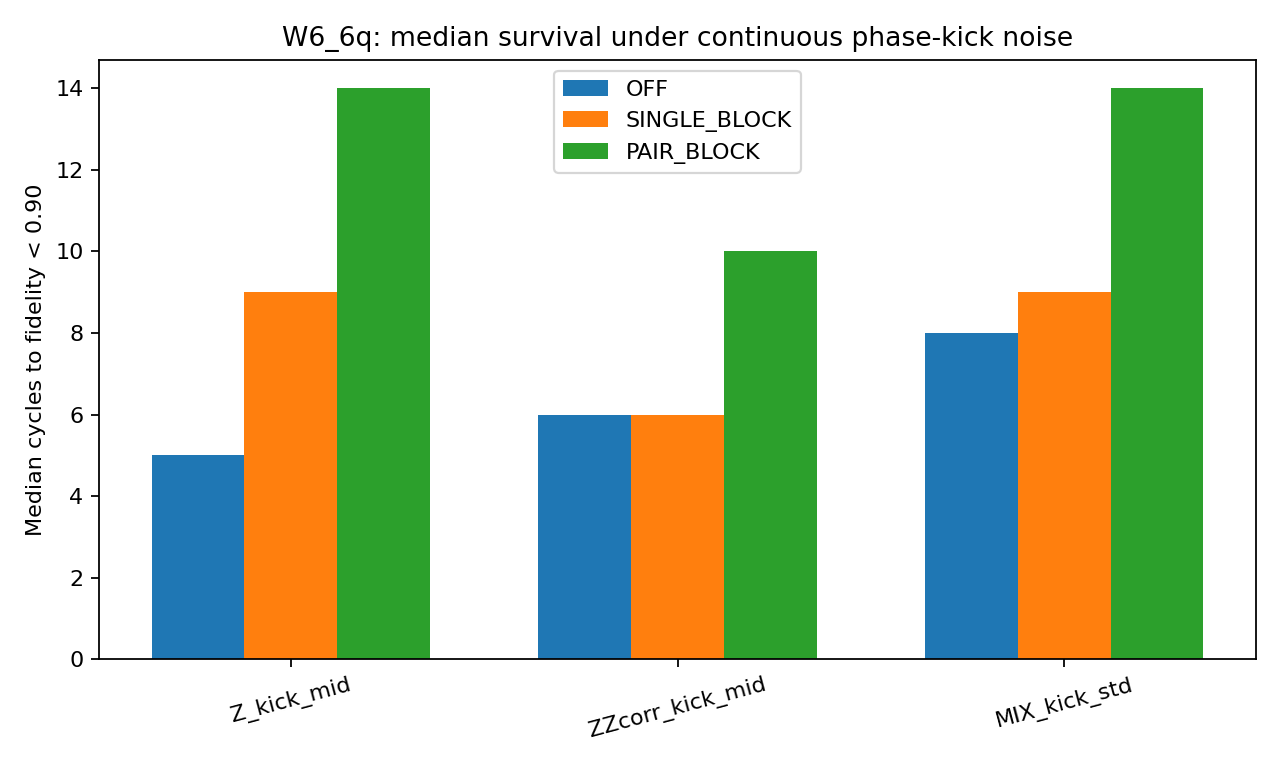
\includegraphics[width=0.9\textwidth,height=\textheight]{figures/W6_6q_median_bars.png}
\caption{W6\_6q median cycles-to-threshold by noise condition and
controller mode.}
\end{figure}

\begin{figure}
\centering
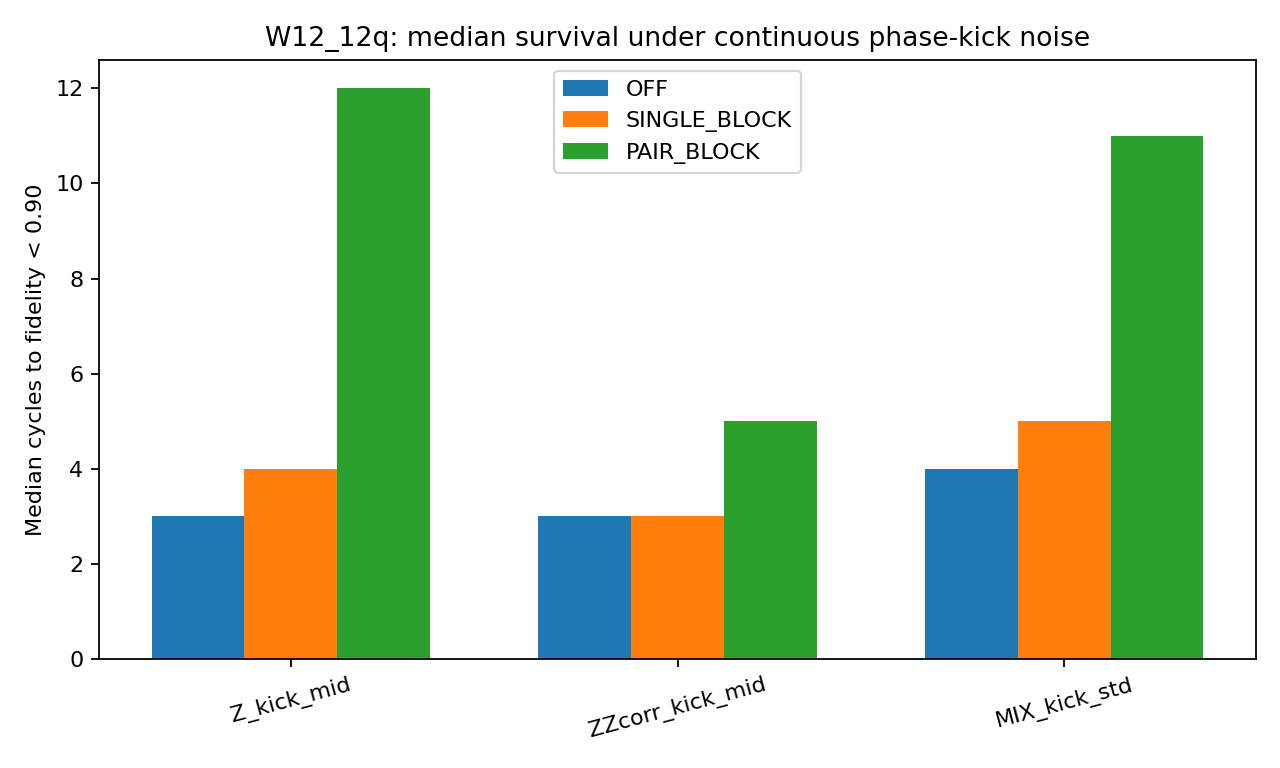
\includegraphics[width=0.9\textwidth,height=\textheight]{figures/W12_12q_median_bars.png}
\caption{W12\_12q median cycles-to-threshold by noise condition and
controller mode.}
\end{figure}

\begin{figure}
\centering
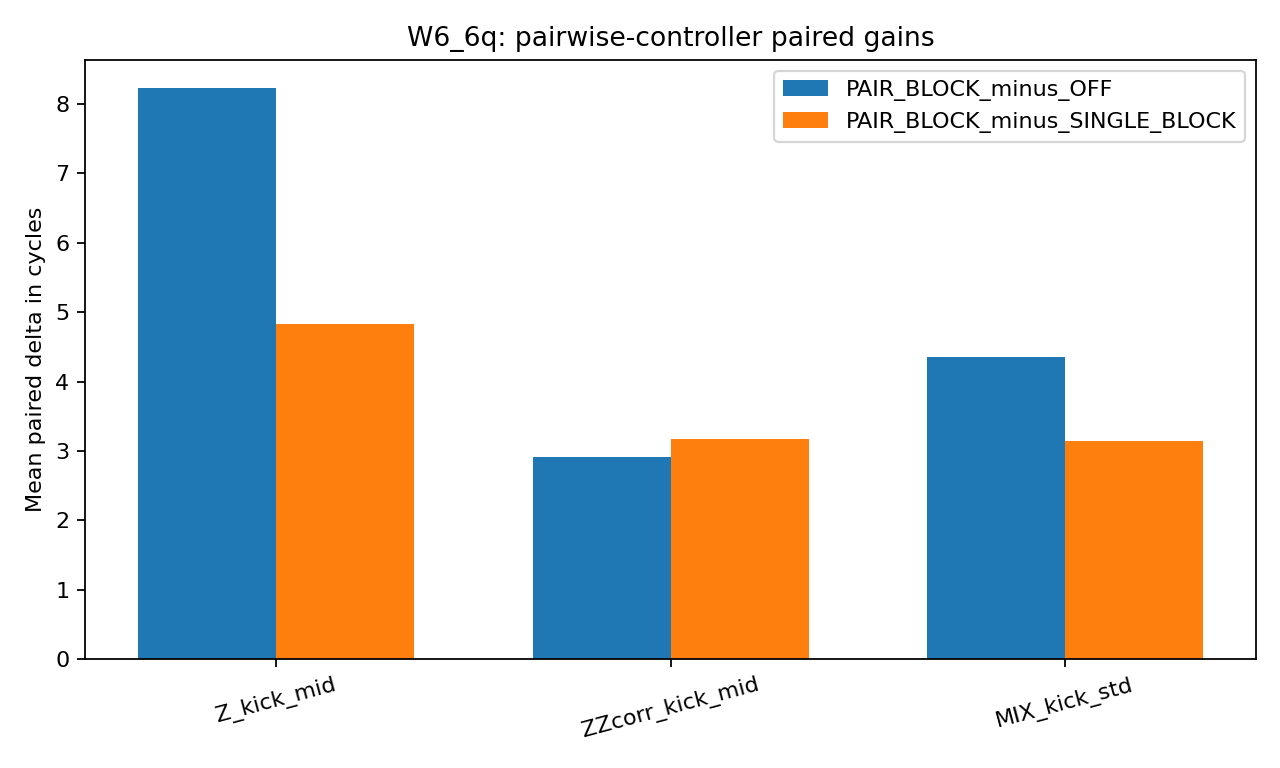
\includegraphics[width=0.9\textwidth,height=\textheight]{figures/W6_6q_pairwise_deltas.png}
\caption{W6\_6q paired deltas for PAIR\_BLOCK relative to OFF and
SINGLE\_BLOCK.}
\end{figure}

\begin{figure}
\centering
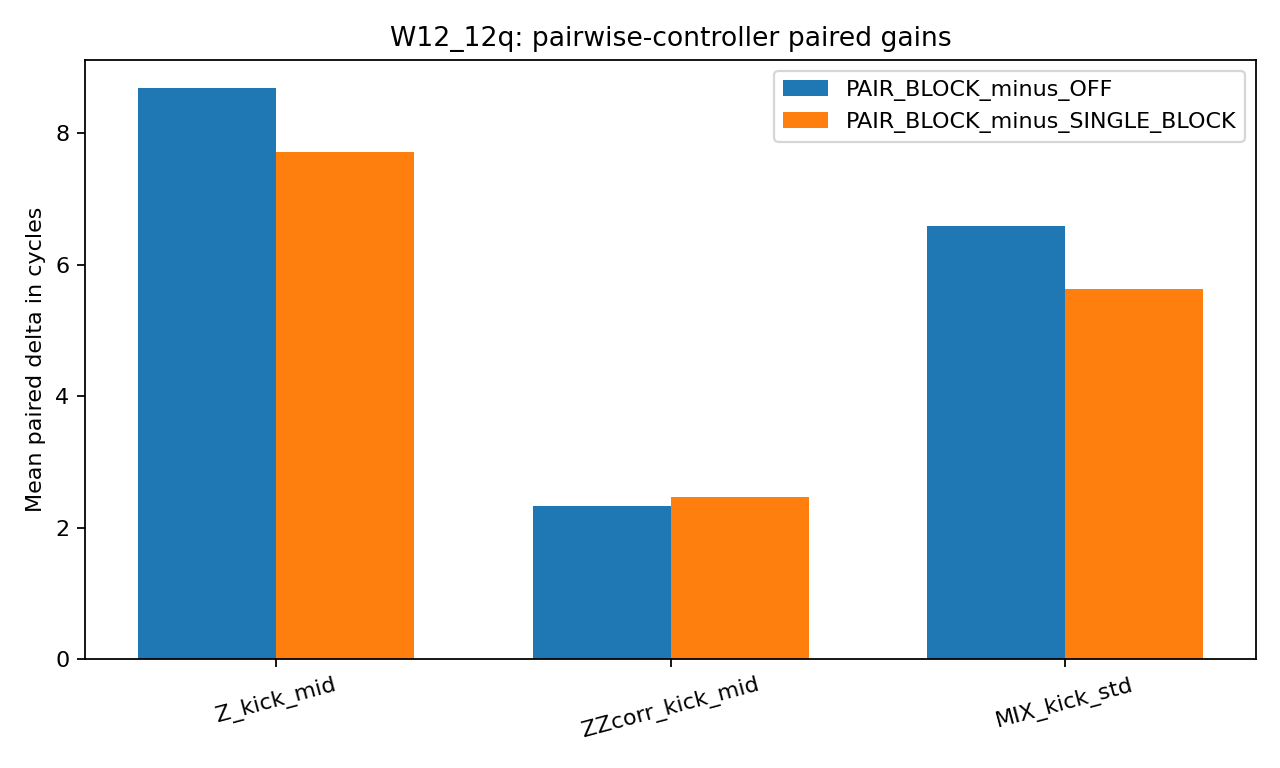
\includegraphics[width=0.9\textwidth,height=\textheight]{figures/W12_12q_pairwise_deltas.png}
\caption{W12\_12q paired deltas for PAIR\_BLOCK relative to OFF and
SINGLE\_BLOCK.}
\end{figure}

\subsubsection{5.4 Sensitivity pass}\label{sensitivity-pass}

The separate 80-seed sensitivity pass preserved the direction of the
main OFF-versus-PAIR\_BLOCK median separation in every tested
workload/noise combination. The preserved median values from the
sensitivity file were:

\begin{itemize}
\tightlist
\item
  W6\_6q, Z\_kick\_mid: OFF 5, PAIR\_BLOCK 14.
\item
  W6\_6q, ZZcorr\_kick\_mid: OFF 6, PAIR\_BLOCK 10.
\item
  W6\_6q, MIX\_kick\_std: OFF 8, PAIR\_BLOCK 14.
\item
  W12\_12q, Z\_kick\_mid: OFF 3, PAIR\_BLOCK 12.
\item
  W12\_12q, ZZcorr\_kick\_mid: OFF 3, PAIR\_BLOCK 5.
\item
  W12\_12q, MIX\_kick\_std: OFF 4.5, PAIR\_BLOCK 11.
\end{itemize}

This pass does not replace the main paired analysis, but it does show
that the observed direction of effect did not reverse under a fresh set
of seeds.

\subsection{6. Interpretation}\label{interpretation}

The saved simulation outputs support the following narrow reading.

\begin{enumerate}
\def\labelenumi{\arabic{enumi}.}
\tightlist
\item
  In this measurement-limited statevector simulation, nearest-neighbor
  pairwise summaries were more informative for active control under
  continuous phase-kick noise than single-qubit summaries alone.
\item
  The difference was largest under independent continuous Z kicks,
  remained visible under mixed phase-kick noise, and was smaller under
  nearest-neighbor ZZ kicks.
\item
  The result is an observation about the simulation design that was run.
  It does not establish hardware performance, universal controller
  superiority, a compiler/runtime advantage, or a general statement
  about all noise models.
\end{enumerate}

The value of the result lies in explanation: when the perturbation
rotates local observables into edge observables, the edge observables
contain control-relevant information. The pairwise controller had access
to that information; the single-summary controller did not.

\subsection{7. Limitations}\label{limitations}

This study has several important limits.

\begin{itemize}
\tightlist
\item
  It is a \textbf{statevector simulation}, not a hardware experiment.
\item
  The controller is \textbf{measurement-limited}, but it is still
  \textbf{model-guided}, because it compares measured summaries with
  ideal target summaries.
\item
  The released package reproduces \textbf{analysis from preserved
  run-level CSV files}. It does \textbf{not} reconstruct the full
  simulator source that originally generated those files.
\item
  The noise model is a \textbf{continuous phase-kick model} with fixed
  Gaussian parameters and a low-rate X-flip component in the mixed
  condition. Results should not be extrapolated beyond those settings
  without rerunning the simulator.
\item
  The archived bootstrap intervals are percentile intervals computed
  from the preserved paired deltas. They summarize the retained run set;
  they do not substitute for a fresh end-to-end rerun.
\end{itemize}

\subsection{8. Reproducibility}\label{reproducibility}

The package accompanying this manuscript contains:

\begin{itemize}
\tightlist
\item
  run-level data (\texttt{pairwise\_runs.csv}),
\item
  aggregate summaries (\texttt{pairwise\_summary.csv}),
\item
  paired comparison tables (\texttt{pairwise\_comparisons.csv}),
\item
  entropy sensitivity summaries (\texttt{entropy\_sensitivity.csv}),
\item
  the preserved analysis script
  (\texttt{scripts/reproduce\_analysis.py}),
\item
  figure files used in this manuscript.
\end{itemize}

A reader can reproduce the tables and descriptive statistics reported
here directly from the included CSV files. What cannot be reproduced
from the archived package alone is the original simulator execution path
that created the run files, because that source was not preserved with
the artifact bundle.

\subsection{Acknowledgments}\label{acknowledgments}

Drafting and formatting support for this manuscript were assisted by
ChatGPT (OpenAI GPT-5.4 Thinking). The author reviewed and approved the
final text.

\subsection{References}\label{references}

{[}1{]} H. M. Wiseman, ``Quantum theory of continuous feedback,''
\emph{Physical Review A} \textbf{49}, 2133-2150 (1994). DOI:
10.1103/PhysRevA.49.2133.

{[}2{]} H. M. Wiseman and G. J. Milburn, \emph{Quantum Measurement and
Control}. Cambridge University Press (2009).

{[}3{]} C. Sayrin, I. Dotsenko, X. Zhou, B. Peaudecerf, T. Rybarczyk, S.
Gleyzes, P. Rouchon, M. Mirrahimi, H. Amini, M. Brune, J.-M. Raimond,
and S. Haroche, ``Real-time quantum feedback prepares and stabilizes
photon number states,'' \emph{Nature} \textbf{477}, 73-77 (2011). DOI:
10.1038/nature10376.

{[}4{]} R. Vijay, C. Macklin, D. H. Slichter, S. J. Weber, K. W. Murch,
R. Naik, A. N. Korotkov, and I. Siddiqi, ``Stabilizing Rabi oscillations
in a superconducting qubit using quantum feedback,'' \emph{Nature}
\textbf{490}, 77-80 (2012). DOI: 10.1038/nature11505.

{[}5{]} B. Efron and R. J. Tibshirani, \emph{An Introduction to the
Bootstrap}. Chapman and Hall/CRC (1993).

{[}6{]} T. J. Evans, R. Harper, and S. T. Flammia, ``Scalable Bayesian
Hamiltonian Learning,'' arXiv:1912.07636 (2019).

\subsection{Appendix A. File
inventory}\label{appendix-a.-file-inventory}

\begin{itemize}
\tightlist
\item
  \texttt{data/pairwise\_runs.csv}
\item
  \texttt{data/pairwise\_summary.csv}
\item
  \texttt{data/pairwise\_comparisons.csv}
\item
  \texttt{data/entropy\_sensitivity.csv}
\item
  \texttt{paper/figures/W6\_6q\_median\_bars.png}
\item
  \texttt{paper/figures/W12\_12q\_median\_bars.png}
\item
  \texttt{paper/figures/W6\_6q\_pairwise\_deltas.png}
\item
  \texttt{paper/figures/W12\_12q\_pairwise\_deltas.png}
\item
  \texttt{scripts/reproduce\_analysis.py}
\end{itemize}

\subsection{Appendix B. Minimal reproduction
workflow}\label{appendix-b.-minimal-reproduction-workflow}

\begin{enumerate}
\def\labelenumi{\arabic{enumi}.}
\tightlist
\item
  Create a Python environment with \texttt{pandas} and \texttt{numpy}.
\item
  Run \texttt{python\ scripts/reproduce\_analysis.py}.
\item
  Verify that the regenerated aggregate tables match the CSV summaries
  in \texttt{data/}.
\item
  Review the figures in \texttt{paper/figures/} against the table
  values.
\end{enumerate}

\end{document}
